% !TeX root = ../main.tex
% 原始章节：17-chip-backend.Rmd

\chapter{芯片后端实现}\label{chap:17-chip-backend}

本章内容将根据后端流程、物理实现（布局布线等）、时序signoff（静态时序分析）、功耗与IR signoff、物理验证五个部分进行描述。

\section{芯片后端设计流程}\label{sec:17-chip-backend-001}

芯片后端设计流程是芯片设计过程中至关重要的环节，它涵盖了从前端设计完成后的电路布局、布线、物理实现及验证的全部工作。

芯片后端设计流程主要包括以下几个阶段：

\begin{itemize}
\tightlist
\item
  设计规划：这个阶段一般在芯片项目初期完成，明确芯片合适的工艺节点、性能、面积功耗范围等。同时，还需要制定详细的项目计划和时间表。
\item
  逻辑综合：如第16.5节所述，逻辑综合是将高级语言描述的逻辑设计转化为门级网表的过程，生成的门级网表将作为后续布局布线的输入（这一步也可以认为是前端综合的工作）。
\item
  \textbf{布局规划}：布局规划是芯片后端设计的重要环节，它决定了芯片中各个元件的位置和布局。在这个阶段，需要考虑芯片的尺寸规划、IO 规划、macro 摆放、物理单元插入等因素。合理的布局规划可以提高芯片的性能、降低功耗、减小面积。

  \begin{itemize}
  \tightlist
  \item
    芯片尺寸规划：芯片尺寸规划需要根据芯片的功能需求和性能指标来确定。一般来说，芯片尺寸越大，能够容纳的元件越多，但成本也会相应增加。在进行芯片尺寸规划时，需要考虑到工艺节点、封装形式、散热要求等因素。
  \item
    IO 规划：IO 规划是确定芯片输入输出端口的位置和数量。合理的 IO 规划可以提高芯片的易用性和可靠性。在进行 IO 规划时，需要考虑到信号完整性、电源完整性、封装要求等因素。
  \item
    Macro 摆放：Macro 摆放是将宏单元（如存储器、处理器核等）放置在芯片中的合适位置。Macro 的摆放需要考虑到信号传输的路径、功耗分布、散热要求等因素。
  \item
    物理单元插入：物理单元插入是在芯片中插入一些特殊的物理单元，如电源网格、时钟树单元等，以提高芯片的性能和可靠性。在进行物理单元插入时，需要考虑到工艺节点、设计约束、信号完整性等因素。
  \end{itemize}
\item
  \textbf{时钟树综合}：时钟树综合是构建时钟信号的传输网络，确保时钟信号的准确性和稳定性。时钟树综合的基本步骤包括确定时钟源和时钟目标、设计时钟树结构、调整时钟树的延迟和偏差等。
\item
  \textbf{布线}：布线是连接芯片中的各个元件，实现信号的传输。布线的基本步骤包括全局布线、详细布线、布线优化等。
\item
  \textbf{物理验证}：物理验证是检查芯片的设计是否符合制造工艺的要求，如 DRC（设计规则检查）、LVS（版图与原理图一致性检查）、Antenna 检查等。物理验证的目的是确保芯片的设计能够在制造过程中顺利实现，并且具有良好的性能和可靠性。
\item
  \textbf{时序分析}：时序分析是分析芯片的时序性能，确保满足设计要求。时序分析的基本步骤包括提取时序模型、进行静态时序分析（STA）、修复时序违规等。在物理实现的各个阶段以及最终的signoff，STA都需要进行以确保每一步的时序都满足要求。
\item
  \textbf{功耗分析}：功耗分析是评估芯片的功耗，进行优化以降低功耗。功耗分析的基本步骤包括功耗建模、功耗评估、功耗优化等。合理的功耗分析可以降低芯片的功耗，提高芯片的可靠性和稳定性。
\item
  \textbf{最终输出}：最终输出是生成用于制造芯片的 GDSII 文件。GDSII 文件包含了芯片的物理信息，如元件的位置、形状、连接关系等。在生成 GDSII 文件之前，需要进行最后的检查和验证，确保芯片的设计符合制造工艺的要求。
\end{itemize}

\section{芯片物理设计}\label{sec:17-chip-backend-002}

\subsection{设计初始化}\label{sec:17-chip-backend-003}

后端设计需要的库文件主要包括工艺库、IP库和设计约束文件等。 工艺库提供了制造芯片所需的各种物理信息，如晶体管的尺寸、电容电阻值、工艺规则等。工艺库是芯片物理设计的基础，它涵盖了芯片的性能、功耗、面积等关键信息。

IP库包含了预先设计好的功能模块，可以直接在设计中使用。IP库可以提高芯片设计的效率和质量，减少设计时间和成本。例如，IP库中的存储器等模块可以直接集成到芯片设计中，无需重新设计。

设计约束文件则规定了芯片的性能要求，如时序约束、面积约束、功耗约束等。设计约束文件是芯片物理设计的指导，它决定了芯片的设计方向和优化目标。例如，设计约束文件中的时序约束规定了芯片中各个信号的传输时间和延迟要求，设计人员需要根据这些约束进行布局布线和时序优化，以确保芯片的时序性能满足设计要求。

以 Innovus 为例，数据初始化的步骤如下：

\begin{itemize}
\item
  导入工艺库和设计约束文件。在 Innovus 中，可以通过菜单栏中的 ``File''-\textgreater{}``Import''-\textgreater{}``Library'' 和 ``File''-\textgreater{}``Import''-\textgreater{}``Constraints'' 分别导入工艺库和设计约束文件。
\item
  创建设计项目，设置芯片的基本参数，如芯片尺寸、工艺节点等。在 Innovus 中，可以通过菜单栏中的 ``File''-\textgreater{}``New''-\textgreater{}``Project'' 创建设计项目，并在项目设置中设置芯片的基本参数。
\item
  导入逻辑网表，进行初步的布局规划。在 Innovus 中，可以通过菜单栏中的 ``File''-\textgreater{}``Import''-\textgreater{}``Netlist'' 导入逻辑网表，并使用布局规划工具进行初步的布局规划。
\end{itemize}

\subsection{布局规划}\label{sec:17-chip-backend-004}

芯片尺寸规划需要根据芯片的功能需求和性能指标来确定。一般来说，芯片尺寸越大，能够容纳的元件越多，但成本也会相应增加。在进行芯片尺寸规划时，需要考虑到工艺节点、封装形式、散热要求等因素。例如，对于高性能的处理器芯片，需要较大的芯片尺寸来容纳更多的晶体管和缓存，但同时也需要考虑到散热问题，避免芯片过热导致性能下降。

IO 规划是确定芯片输入输出端口的位置和数量。合理的 IO 规划可以提高芯片的易用性和可靠性。在进行 IO 规划时，需要考虑到信号完整性、电源完整性、封装要求等因素。例如，对于高速数据传输的芯片，需要合理规划 IO 端口的位置和数量，以确保信号的完整性和稳定性。

Macro 摆放是将宏单元（如存储器、处理器核等）放置在芯片中的合适位置。Macro 的摆放需要考虑到信号传输的路径、功耗分布、散热要求等因素。合理的 Macro 摆放可以提高芯片的性能、降低功耗、减小面积。例如，对于处理器芯片，需要将处理器核放置在芯片的中心位置，以减少信号传输的延迟；同时，需要将存储器放置在靠近处理器核的位置，以提高数据访问的速度。

物理单元插入是在芯片中插入一些特殊的物理单元，如电源网格、时钟树单元等，以提高芯片的性能和可靠性。在进行物理单元插入时，需要考虑到工艺节点、设计约束、信号完整性等因素。例如，电源网格的插入可以提高芯片的电源稳定性，减少电压降和噪声；时钟树单元的插入可以提高芯片的时钟信号的准确性和稳定性，减少时钟偏移和抖动。

一般布局规划的主要目标为：

\begin{itemize}
\item 确定芯片面积：一般芯片的面积越小，平均到每个芯片上的成本越小；但芯片的面积也不可太小，则会造成拥塞程度高，难以布线，导致长周期的设计迭代。一个合理的面积设定是在保证布线的同时尽量节约产品成本，所以布局的最初目标是估计芯片面积的大小。
\item 确保时序收敛：通过优化关键路径、控制信号线长度和时钟树综合，确保信号在规定的时钟周期内传输完成，满足时序要求。
\item 保证芯片的稳定：通过合理的电源和地线规划、热管理和功耗控制，确保芯片在长期运行中保持稳定，防止过热、IR Drop和信号干扰等问题。
\item 满足布线的要求：预留足够的布线资源和空间，采用层次化布线策略，确保布线通畅、信号完整性得到保障，并满足制造工艺的可行性要求。
\end{itemize}


在层次化设计中，由于只在子模块进行时钟树综合，因此需要再布局规划阶段对时钟树上的延迟进行预估和分配。即根据时钟周期，计算时钟在芯片内的延时。如图\ref{fig:chip-place-time}所示。

\begin{figure}[htbp]
  \centering
  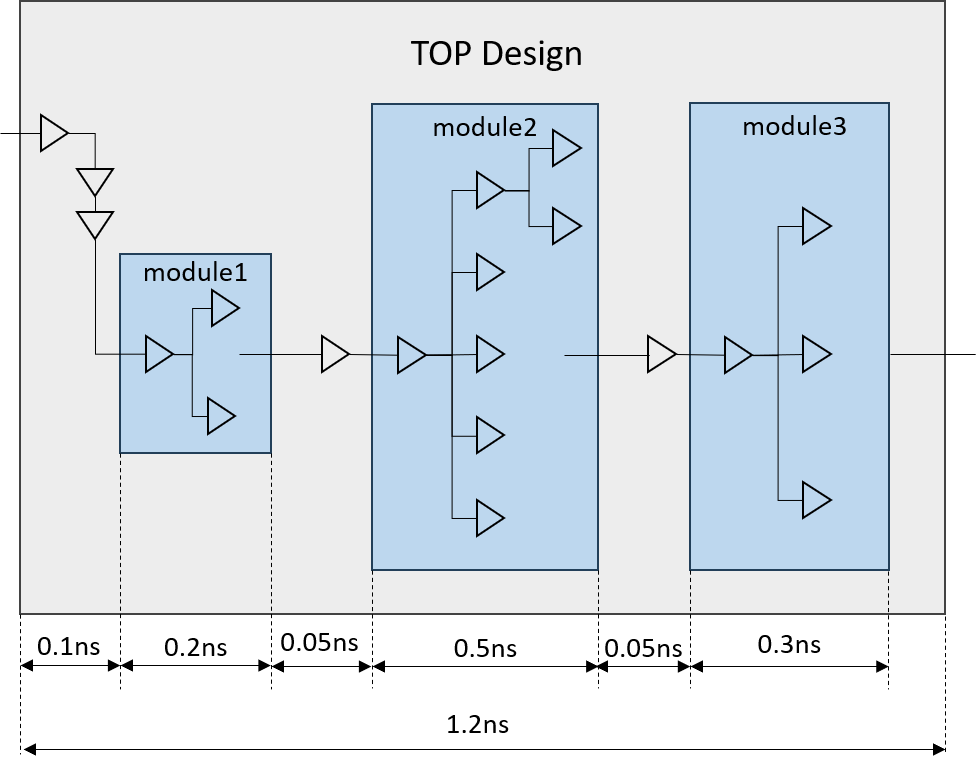
\includegraphics[width=0.8\linewidth]{assets/17/布局规划考虑时钟树延时.png}
  \caption{层次化设计中的布局规划对时钟树延迟的预分配}
  \label{fig:chip-place-time}
\end{figure}

\subsection{电源规划}\label{sec:17-chip-backend-005}

电源规划的简单原理是为芯片中的各个元件提供稳定的电源供应。芯片中的各个元件需要不同的电源电压和电流，因此需要设计合理的电源网络来满足这些需求。电源规划的基本设置包括确定电源电压、电流需求，设计电源网格等。

电源网格是由金属线组成的网络，用于将电源从电源引脚传输到芯片中的各个元件。电源网格的设计需要考虑到电流密度、电压降等因素，以确保电源供应的稳定性。例如，对于高性能的处理器芯片，需要设计密集的电源网格，以满足大电流的需求；同时，需要控制电源网格的电阻和电感，以减少电压降和噪声。

\subsection{自动布局和时序、功耗、面积优化}\label{sec:17-chip-backend-006}

自动布局是利用EDA工具自动将标准单元放置在芯片中的合适位置。在前面手动完成布局规划之后，由EDA工具考虑时序、功耗、面积等因素优化完成自动布局任务。自动布局可以提高设计效率，减少人工干预，同时也可以提高设计的质量和可靠性。

时序优化的目的是确保芯片的时序性能满足设计要求。基本设置包括设置时序约束、调整时钟树结构等。时序优化可以通过调整布局、布线、时钟树等方式来实现。例如，可以通过调整标准单元的位置和方向，减少信号传输的延迟；可以通过调整时钟树的结构和延迟，减少时钟偏移和抖动。

功耗优化的方法包括降低电压、减少开关活动等。功耗优化可以通过调整电源电压、优化电路设计、减少不必要的开关活动等方式来实现。例如，可以通过降低电源电压，减少静态功耗；可以通过优化电路设计，减少动态功耗。

面积优化可以通过压缩布局、优化布线等方式实现。面积优化可以减少芯片的面积，降低成本，同时也可以提高芯片的性能和可靠性。例如，可以通过压缩标准单元的布局，减少芯片的面积；可以通过优化布线，减少布线长度和交叉，提高信号传输的质量。

上述优化一般由EDA工具辅助完成。

\subsection{时钟树综合}\label{sec:17-chip-backend-007}

时钟树综合是构建时钟信号的传输网络，确保时钟信号的准确性和稳定性。时钟树综合工具会将某个同步设计中的时钟信号到达各个终端节点的时间相同，示意图如图\ref{fig:CTS}所示。

\begin{figure}[htbp]
  \centering
  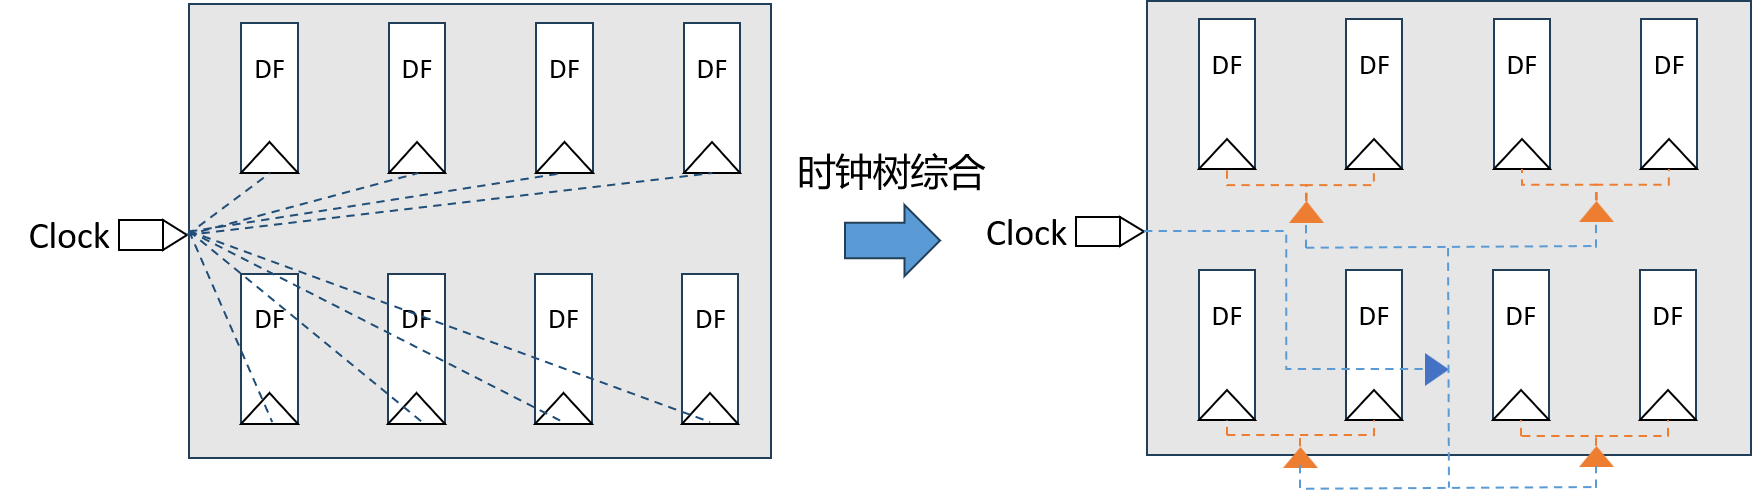
\includegraphics[width=1\linewidth]{assets/17/时钟树综合.png}
  \caption{时钟树综合示意图}
  \label{fig:CTS}
\end{figure}

时钟树综合的基本步骤包括：

确定时钟源和时钟目标。时钟源通常是芯片中的晶振或外部时钟输入，时钟目标是芯片中的各个寄存器和触发器。

设计时钟树结构，如 H 树、鱼骨形等，如上图中就是H树形结构。时钟树结构的选择需要考虑到芯片的面积、功耗、时序等因素。

调整时钟树的延迟和偏差，满足时序约束。时钟树的延迟和偏差需要根据设计约束进行调整，以确保时钟信号的准确性和稳定性。

例如，对于高性能的处理器芯片，需要设计低延迟、低偏差的时钟树结构，以提高时钟信号的准确性和稳定性；同时，需要考虑到时钟树的功耗和面积，避免过度设计。

\subsection{布线}\label{sec:17-chip-backend-008}

布线是连接芯片中的各个元件，实现信号的传输。布线的基本步骤包括：

全局布线：确定信号的大致路径。全局布线通常采用基于 Steiner 树的算法，以最小化布线长度和交叉。

详细布线：精确地连接各个元件。详细布线通常采用基于迷宫算法或 Dijkstra 算法的工具，以确保信号的完整性和稳定性。

布线优化：调整布线的长度、宽度等参数，提高信号传输的质量。布线优化可以通过调整布线的电阻、电容、电感等参数，减少信号传输的延迟和噪声。

例如，对于高速数据传输的芯片，需要进行严格的布线优化，以确保信号的完整性和稳定性；同时，需要考虑到布线的功耗和面积，避免过度设计。

\subsection{数据输出}\label{sec:17-chip-backend-009}

芯片物理设计完成后，需要输出用于制造芯片的 GDSII 文件。GDSII 文件包含了芯片的物理信息，如元件的位置、形状、连接关系等。在输出 GDSII 文件之前，需要进行最后的检查和验证，确保芯片的设计符合制造工艺的要求。

例如，可以使用物理验证工具对 GDSII 文件进行 DRC、LVS、Antenna 检查等，确保芯片的设计没有违反制造工艺的规则；可以使用时序分析工具对芯片的时序性能进行最后的验证，确保芯片的时序性能满足设计要求。

\section{芯片时序 signoff}\label{sec:17-chip-backend-010}

芯片时序 signoff 的流程包括：

提取时序模型：从物理设计中提取出用于时序分析的模型。时序模型通常包括晶体管级模型、门级模型、寄存器传输级模型等。提取时序模型的工具可以采用静态时序分析（STA）工具或动态时序分析（DTA）工具，但由于DTA的时间一般要远大于STA的时间，因此一般选用STA作为分析工具。

进行静态时序分析（STA）：检查芯片的时序性能是否满足设计要求。STA 是一种基于模型的分析方法，它通过分析芯片的逻辑结构和物理实现，预测芯片的时序性能。STA 可以快速地检查大量的时序路径，发现潜在的时序问题。

修复时序违规：如果存在时序违规，需要进行优化以修复违规。时序违规的修复通常采用调整布局、布线、时钟树等方式来实现。例如，可以通过调整标准单元的位置和方向，减少信号传输的延迟；可以通过调整时钟树的结构和延迟，减少时钟偏移和抖动。

生成时序报告：记录时序分析的结果，供设计人员参考。时序报告通常包括时序路径的延迟、时钟偏移、建立时间和保持时间等信息。

检查内容主要包括：

建立时间和保持时间检查：确保数据在时钟信号的上升沿和下降沿能够正确地被锁存。建立时间是指数据在时钟信号上升沿之前必须稳定的时间，保持时间是指数据在时钟信号上升沿之后必须稳定的时间。

时钟偏移检查：检查时钟信号在不同路径上的延迟差异。时钟偏移是指时钟信号在不同路径上的延迟差异，它会影响芯片的时序性能。

路径延迟检查：检查信号在不同路径上的传输延迟。路径延迟是指信号在不同路径上的传输延迟，它会影响芯片的时序性能。

静态时序分析（STA）是一种基于模型的分析方法，它通过分析芯片的逻辑结构和物理实现，预测芯片的时序性能。STA 可以快速地检查大量的时序路径，发现潜在的时序问题。STA 的基本原理是将芯片的逻辑结构和物理实现转化为时序图，然后通过分析时序图中的路径延迟、时钟偏移、建立时间和保持时间等信息，判断芯片的时序性能是否满足设计要求。

\section{芯片功耗与 IR signoff}\label{sec:17-chip-backend-011}

芯片功耗与 IR signoff 的流程包括：

功耗分析：评估芯片的功耗，确定功耗是否满足设计要求。功耗分析的方法通常包括静态功耗分析和动态功耗分析。静态功耗分析分析是指在芯片不工作时的功耗，动态功耗分析是指在芯片工作时的功耗。

IR 分析：检查芯片的电源网格是否能够提供稳定的电源供应。IR 分析是指检查芯片的电源网格的电压降和电流密度是否在允许的范围内。如果电源网格的电压降和电流密度超过了允许的范围，可能会导致芯片的性能下降或失效。

优化功耗和 IR：如果存在问题，需要进行优化以降低功耗和改善 IR。功耗优化的方法包括降低电压、减少开关活动、优化电路设计等。IR 优化的方法包括调整电源网格的结构、增加电源引脚的数量、降低电源网格的电阻等。

生成功耗和 IR 报告：记录分析的结果，供设计人员参考。功耗和 IR 报告通常包括芯片的功耗、电源网格的电压降和电流密度等信息。

基本原理：

功耗分析主要考虑动态功耗和静态功耗。动态功耗是由芯片中的开关活动引起的，静态功耗是由漏电流等因素引起的。IR 分析是检查电源网格的电压降是否在允许的范围内，以确保芯片能够正常工作。动态功耗的计算公式为 P\_dynamic = C * V\^{}2 * f，其中 C 是电容，V 是电压，f 是频率。静态功耗的计算公式为 P\_static = I\_leakage * V，其中 I\_leakage 是漏电流，V 是电压。IR 分析的基本原理是根据欧姆定律，计算电源网格的电阻和电流，然后根据电阻和电流计算电压降。如果电压降超过了允许的范围，需要进行优化以降低电压降。

\section{物理验证}\label{sec:17-chip-backend-012}

DRC（设计规则检查）

DRC 的流程包括：

定义设计规则：根据制造工艺的要求，定义各种设计规则，如最小线宽、最小间距、最大金属密度等。设计规则是制造芯片的基本要求，违反设计规则可能会导致芯片制造失败。

进行 DRC 检查：使用工具对芯片的物理设计进行检查，确保设计符合设计规则。DRC 检查通常采用自动化工具，如 Calibre、Mentor Graphics 的 DRC 工具等。

修复 DRC 违规：如果存在 DRC 违规，需要进行修改以满足设计规则。DRC 违规的修复通常需要调整布局、布线、金属层等，以确保设计符合制造工艺的要求。

基本原理：DRC 检查是为了确保芯片的物理设计能够在制造过程中顺利实现。制造工艺对芯片的尺寸、间距、金属密度等有严格的要求，如果设计违反了这些要求，可能会导致制造失败。例如，最小线宽和最小间距的要求是为了确保金属线之间有足够的空间，避免短路和漏电；最大金属密度的要求是为了确保芯片在制造过程中不会出现过度蚀刻或过度填充的问题。

LVS（版图与原理图一致性检查）

LVS 的流程包括：

提取原理图和版图信息：分别从逻辑设计和物理设计中提取出原理图和版图信息。原理图信息通常包括电路的逻辑连接关系、元件的参数等；版图信息通常包括芯片的物理布局、金属层的连接关系等。可以使用专门的提取工具来完成这一步骤，确保信息的准确性和完整性。

进行 LVS 检查：比较原理图和版图的连接关系，确保它们是一致的。这一步骤通常使用自动化的 LVS 工具，该工具会对原理图和版图中的各个节点、元件进行逐一对比，检查它们的连接关系、属性等是否匹配。如果发现不一致的地方，工具会生成详细的报告，指出具体的问题所在。

修复 LVS 违规：如果存在 LVS 违规，需要进行修改以确保原理图和版图的一致性。根据 LVS 报告中的问题描述，设计人员需要仔细分析违规的原因，并采取相应的措施进行修复。可能需要调整版图布局、修改电路连接或者更新元件参数等。修复完成后，再次进行 LVS 检查，直到所有问题都得到解决。

基本原理：LVS 检查是为了确保芯片的物理设计与逻辑设计是一致的。如果物理设计与逻辑设计不一致，可能会导致芯片的功能错误。在芯片设计过程中，逻辑设计和物理设计是两个不同的阶段，分别由不同的工具和人员进行。由于各种原因，可能会出现逻辑设计与物理设计不一致的情况，例如在布局布线过程中出现错误连接、元件参数设置错误等。LVS 检查通过比较原理图和版图的连接关系，可以及时发现这些问题，并进行修复，从而保证芯片的正确性和可靠性。

Antenna 检查

Antenna 检查的流程包括：

识别天线结构：在物理设计中识别可能存在天线效应的结构。天线效应是指在制造过程中，芯片中的金属线可能会像天线一样收集电荷，导致晶体管的栅极被击穿。一些较长的金属线、未连接到地的金属结构等都可能成为天线结构。可以使用专门的 Antenna 检查工具来识别这些结构。

计算天线比率：计算天线结构的天线比率，判断是否超过允许的范围。天线比率是指天线结构收集的电荷与晶体管栅极电容的比值。如果天线比率超过了允许的范围，就可能导致栅极被击穿。工具会根据制造工艺的要求，计算每个天线结构的比率，并与允许的范围进行比较。

修复 Antenna 问题：如果天线比率超过允许的范围，需要进行修改以降低天线比率。常见的修复方法包括增加接地连接、插入二极管、调整金属层布局等。设计人员需要根据具体情况选择合适的修复方法，并确保修复后的设计满足制造工艺的要求。再次进行 Antenna 检查，直到所有问题都得到解决。

基本原理：在制造过程中，芯片中的金属线可能会像天线一样收集电荷，导致晶体管的栅极被击穿。Antenna 检查是为了确保芯片的物理设计不会引起天线效应，从而保证芯片的可靠性。当芯片在制造过程中暴露在等离子体环境中时，金属线会收集电荷。如果电荷积累到一定程度，就会超过晶体管栅极的耐压能力，导致栅极被击穿。Antenna 检查通过识别可能存在天线效应的结构，并计算天线比率，可以及时发现潜在的问题，并采取相应的措施进行修复，从而避免芯片在制造过程中出现故障。
